\section{Introduction}
The recent advancements in Large Language Models (LLMs) have demonstrated that the quality of language generation significantly improves with an increase in model size, reaching billions of parameters~\citep{brown2020language,chowdhery2022palm,zhang2022opt,hoffmann2022training,openai2023gpt4,google2023palm2,touvron2023llama}. However, this growth has led to an increase in \emph{inference latency}, which poses a significant challenge in practical applications. From a system perspective, LLM inference is predominantly memory-bandwidth-bound~\citep{shazeer2019fast,kim2023squeezellm}, with the main latency bottleneck stemming from accelerators' memory bandwidth rather than arithmetic computations. This bottleneck is inherent to the sequential nature of auto-regressive decoding, where each forward pass requires transferring the complete model parameters from High-Bandwidth Memory (HBM) to the accelerator's cache. This process, which generates only a single token, underutilizes the arithmetic computation potential of modern accelerators, leading to inefficiency.

To address this, one approach to speed up LLM inference involves \emph{increasing the arithmetic intensity} (the ratio of total floating-point operations (FLOPs) to total data movement) of the decoding process and \emph{reducing the number of decoding steps}. In line with this idea, speculative decoding has been proposed~\citep{leviathan2022fast,chen2023accelerating,xia2023speculative,miao2023specinfer}. This method uses a smaller draft model to generate a token sequence, which is then refined by the original, larger model for acceptable continuation. However, obtaining an appropriate draft model remains challenging, and it's even harder to integrate the draft model into a distributed system~\citep{chen2023accelerating}.

Instead of using a separate draft model to sequentially generate candidate outputs, in this paper, we revisit and refine the concept of using multiple decoding heads on top of the backbone model to expedite inference~\citep{stern2018blockwise}. We find that when applied effectively, this technique can overcome the challenges of speculative decoding, allowing for seamless integration into existing LLM systems. Specifically, we introduce \ours, a method that enhances LLM inference by integrating additional decoding heads to concurrently predict multiple tokens. These heads are fine-tuned in a \emph{parameter-efficient} manner and can be added to any existing model. With no requirement for a draft model, \ours offers easy integration into current LLM systems, including those in distributed environments, ensuring a user-friendly experience.

We further enhance \ours with two key insights. Firstly, the current approach of generating a single candidate continuation at each decoding step leads to inefficient use of computational resources. To address this, we propose generating multiple candidate continuations using the \ours heads and verifying them concurrently through a simple adjustment to the attention mask. 
\textcolor{black}{Secondly, we can reuse the rejection sampling scheme as used in speculative decoding~\cite{leviathan2022fast,chen2023accelerating} to generate consistent responses with the same distribution as the original model. However, it cannot further enhance the acceleration rate.}
Alternatively, we introduce a \emph{typical acceptance} scheme that selects \emph{reasonable} candidates from the \ours head outputs. We use temperature as a threshold to manage deviation from the original model’s predictions, providing an efficient alternative to the rejection sampling method. 
\textcolor{black}{Our results suggest that the proposed typical acceptance scheme can accelerate the decoding speed further while maintaining a similar generation quality.}

To equip LLMs with predictive \ours heads, we propose two distinct fine-tuning procedures tailored to various scenarios. For situations with limited computational resources or when the objective is to incorporate \ours into an existing model without affecting its performance, we recommend \ours-1. This method requires minimal memory and can be further optimized with quantization techniques akin to those in QLoRA~\citep{dettmers2023qlora}, without compromising the generation quality due to the fixed backbone model. However, in \ours-1, the full potential of the backbone model is not utilized. We can further fine-tune it to enhance the prediction accuracy of \ours heads, which can directly lead to a greater speedup.
Therefore, we introduce \ours-2, which is suitable for scenarios with ample computational resources or for direct Supervised Fine-Tuning (SFT) from a base model. 
The key to \ours-2 is a training protocol that enables joint training of the \ours heads and the backbone model without compromising the model’s next-token prediction capability and output quality.
We propose different strategies for obtaining the training datasets depending on the model’s training recipe and dataset availability. When the model is fine-tuned on a public dataset, it can be directly used for \ours. If the dataset is unavailable or the model underwent a Reinforcement Learning with Human Feedback (RLHF)~\citep{ouyang2022training} process, we suggest a self-distillation approach to generate a training dataset for the \ours heads.

Our experiments primarily focus on scenarios with a batch size of one, which is representative of the use case where LLMs are locally hosted for personal use. We test \ours on models of varying sizes and training settings, including Vicuna-7B, 13B (trained with a public dataset), Vicuna-33B~\citep{vicuna2023} (trained with a private dataset\footnote{Upon contacting the authors, this version is experimental and used some different data than Vicuna 7B and 13B.}), and Zephyr-7B (trained with both supervised fine-tuning and alignment). \ours can achieve a speedup of 2.3 to 2.8 times across different prompt types without compromising on the quality of generation.







\begin{figure}[h!]
    \centering
    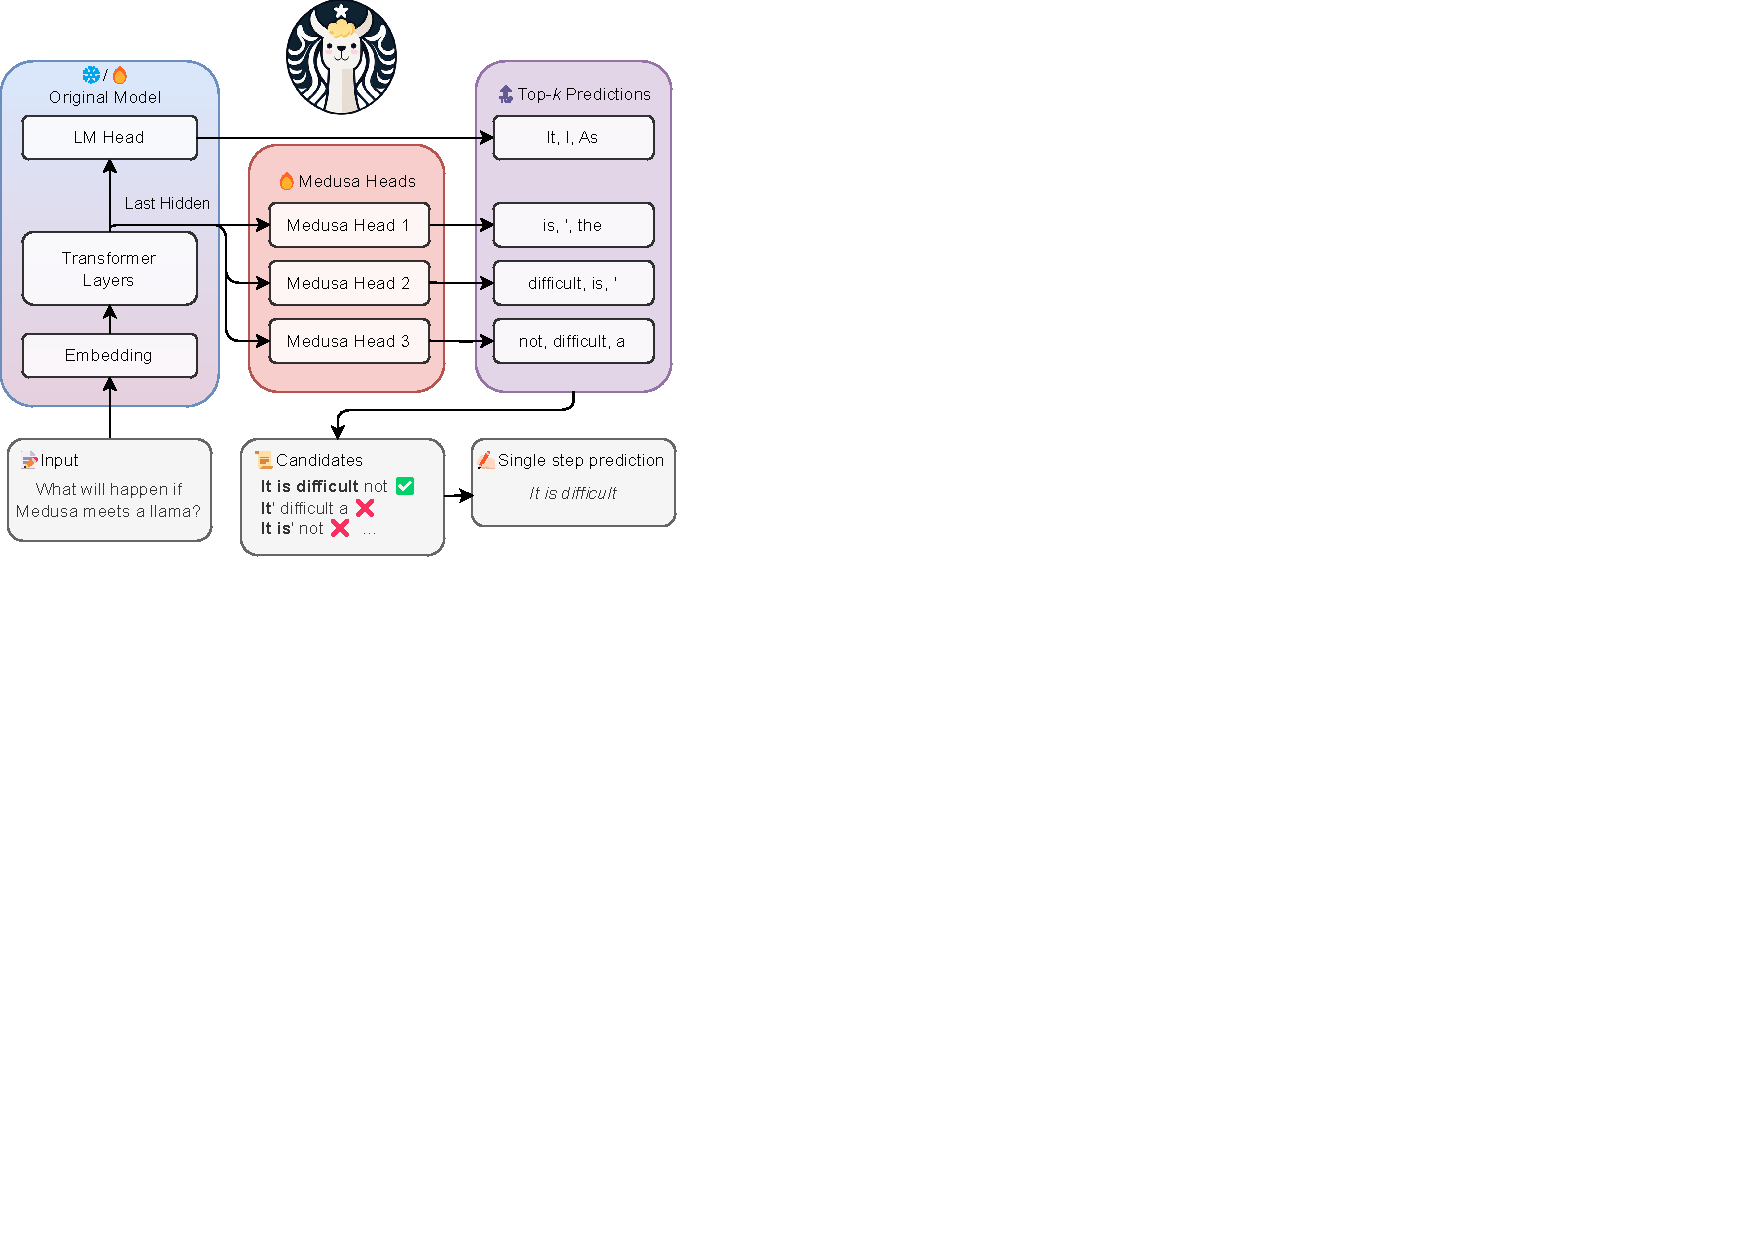
\includegraphics[width=0.45\textwidth]{Medusa.drawio.pdf}
    \caption{
    \ours introduces \emph{multiple heads} on top of the last hidden states of the LLM, enabling the prediction of several subsequent tokens in parallel (Section~\ref{sec:medusa_heads}). 
    During inference, each head generates multiple top predictions for its designated position. 
    These predictions are assembled into candidates, which are processed in parallel using a \emph{tree-based attention} mechanism (Section~\ref{sec:tree_attention}). The final step is to verify the candidates and accept a continuation. Besides the standard rejection sampling scheme, a \emph{typical acceptance} scheme (Section~\ref{sec:typical_acceptance}) can also be used here to select reasonable continuations, and the \emph{longest accepted candidate prefix} will be used for the next decoding phase. 
    }
    \label{fig:pipeline}
\end{figure}